% Gebundene Ströme: atomare Kreisströme heben sich innen auf, außen bleibt K_b = M x n
% Gemeinsamer Stil für alle Abbildungen (TikZ -> SVG, siehe figures/build.mjs).
%
% Farben sind Platzhalter ("Sentinels"): build.mjs ersetzt sie im SVG durch
% CSS-Variablen, damit die Abbildungen im hellen und dunklen Modus passen.
% Andere Farben (auch schwarz/weiß) bricht der Build mit Fehler ab.
%
%   fg    Linien, Beschriftung          -> --dark
%   mu    Hilfslinien, Achsen, Maße      -> --gray
%   acc   das eine Konzept der Abbildung -> --secondary (Lime/Oliv)
%   blue  zweite Größe, negative Ladung  -> --fig-blue
%   warm  dritte Größe, positive Ladung  -> --fig-warm
%   bg    Seitenhintergrund (Aussparen)  -> --light
%
% Kein \clip verwenden: pdftocairo macht daraus Clip-Gruppen, in denen exakt
% waagerechte/senkrechte Linien verschwinden. Berechnete Kurven schneidet
% gen/*.py selbst am Rahmen ab.
\documentclass[tikz,border=3pt]{standalone}
\usepackage{amsmath,amssymb,bm}
% Text serifenlos wie die Seite, Mathe in Computer Modern wie KaTeX
\renewcommand{\familydefault}{\sfdefault}
\usetikzlibrary{arrows.meta,calc,decorations.markings,patterns,3d,positioning,angles,quotes}

\definecolor{fg}{RGB}{1,2,3}
\definecolor{mu}{RGB}{4,5,6}
\definecolor{acc}{RGB}{7,8,9}
\definecolor{blue}{RGB}{10,11,12}
\definecolor{warm}{RGB}{13,14,15}
\definecolor{bg}{RGB}{16,17,18}

% Vektoren wie auf der Website (KaTeX \mathbf)
\newcommand{\vv}[1]{\mathbf{#1}}

\tikzset{
  every picture/.style={fg, line width=0.8pt, line cap=round, line join=round,
    >={Stealth[length=5.5pt,width=4.4pt]}},
  every node/.style={font=\small},
  % Linientypen
  main/.style={line width=0.9pt},
  thin/.style={line width=0.5pt},
  aux/.style={mu, line width=0.5pt, dash pattern=on 2.5pt off 2pt},
  axis/.style={mu, line width=0.6pt, ->},
  vec/.style={line width=1.1pt, ->},
  field/.style={line width=0.7pt, postaction={decorate},
    decoration={markings, mark=at position #1 with {\arrow{Stealth[length=4.5pt,width=3.6pt]}}}},
  field/.default=0.5,
  % Flächen
  soft/.style={fill=#1, fill opacity=0.14},
  soft/.default=acc,
  % Ladungen
  qpos/.style={circle, fill=warm, inner sep=0pt, minimum size=9pt,
    path picture={\draw[bg, line width=0.9pt] ($(path picture bounding box.center)+(-2pt,0)$) -- +(4pt,0)
      ($(path picture bounding box.center)+(0,-2pt)$) -- +(0,4pt);}},
  qneg/.style={circle, fill=blue, inner sep=0pt, minimum size=9pt,
    path picture={\draw[bg, line width=0.9pt] ($(path picture bounding box.center)+(-2pt,0)$) -- +(4pt,0);}},
  dot/.style={circle, fill=fg, inner sep=0pt, minimum size=3pt},
  % Beschriftung mit Aussparung, damit Linien den Text nicht kreuzen
  lbl/.style={fill=bg, inner sep=1.5pt},
  % Icons: kräftigere Linien, keine Schrift
  icon/.style={line width=1.6pt, >={Stealth[length=6pt,width=5pt]}},
}

\begin{document}
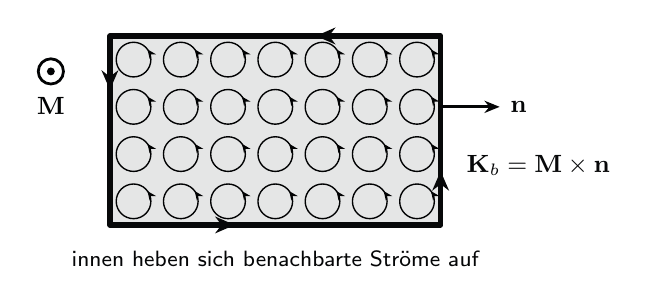
\begin{tikzpicture}
  \def\W{4.2} \def\H{2.4}
  \fill[mu, fill opacity=0.1] (0,0) rectangle (\W,\H);
  % atomare Kreisströme (gegen den Uhrzeigersinn -> m aus der Ebene)
  \foreach \i in {0,...,6} \foreach \j in {0,...,3} {
    \pgfmathsetmacro{\x}{0.3+\i*0.6}
    \pgfmathsetmacro{\y}{0.3+\j*0.6}
    \draw[thin, postaction={decorate}, decoration={markings,
        mark=at position 0.1 with {\arrow{Stealth[length=3.2pt,width=2.8pt]}}}]
      (\x+0.22,\y) arc[start angle=0, end angle=360, radius=0.22];
  }
  % Oberflächenstrom K_b, ebenfalls gegen den Uhrzeigersinn
  \draw[acc, line width=2pt, postaction={decorate}, decoration={markings,
      mark=at position 0.12 with {\arrow{Stealth[length=7pt,width=6pt]}},
      mark=at position 0.37 with {\arrow{Stealth[length=7pt,width=6pt]}},
      mark=at position 0.62 with {\arrow{Stealth[length=7pt,width=6pt]}},
      mark=at position 0.87 with {\arrow{Stealth[length=7pt,width=6pt]}}}]
    (0,0) -- (\W,0) -- (\W,\H) -- (0,\H) -- cycle;
  % rechte Seite: n nach außen, K_b = M x n = ez x ex = ey
  \draw[vec, mu] (\W,1.5) -- (\W+0.75,1.5) node[anchor=west, text=mu] {$\vv n$};
  \node[acc, anchor=west] at (\W+0.2,0.75) {$\vv K_b=\vv M\times\vv n$};
  % M aus der Ebene
  \begin{scope}[shift={(-0.75,1.95)}]
    \draw[line width=1pt] (0,0) circle (0.16);
    \fill (0,0) circle (0.05);
    \node[anchor=north] at (0,-0.2) {$\vv M$};
  \end{scope}
  \node[mu, font=\footnotesize, align=center, anchor=north] at (\W/2,-0.2) {innen heben sich benachbarte Ströme auf};
\end{tikzpicture}
\end{document}
